% Chapter 7

\chapter{Evaluations} % Main chapter title

\label{eval} % For referencing the chapter elsewhere, use \ref{Chapter1} 

\lhead{Chapter 7. \emph{Evaluations}} % This is for the header on each page - perhaps a shortened title

%\section{Conclusion}
%
%\section{Future Work}
%
%\subsection{Summarizing Event Related Content}
%
%\subsection{Identifying Insightful Opinionated Content Related to Events}
%
%\subsection{Event Topic Modeling}
%
%\subsection{Event-specific Recommendations}
%
%\subsection{Distributed Processing of EventIdentityInfoGraph}
%
%\subsection{Event Ontology for Social Media}

\begin{figure}[htbp]
\centering
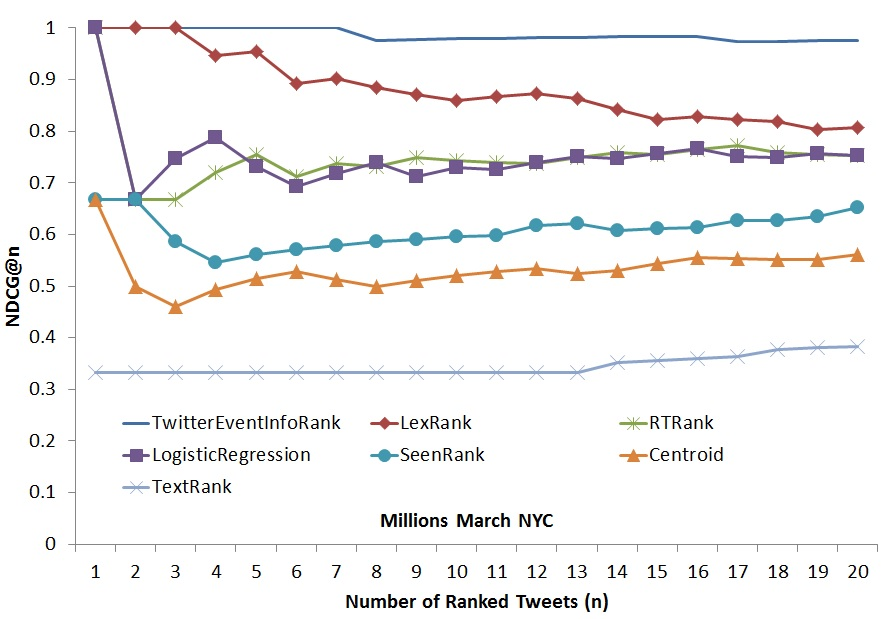
\includegraphics[height=4.5in,width=6in]{Figures/Chapter4Figures/MillionsMarchNycEventIdentityInfoRankPerformance.jpg}
\caption{\small Performance comparison of ranking techniques using NDCG scores.}
\label{millionsmarchndcg}
\end{figure}

\begin{figure}[htbp]
\centering
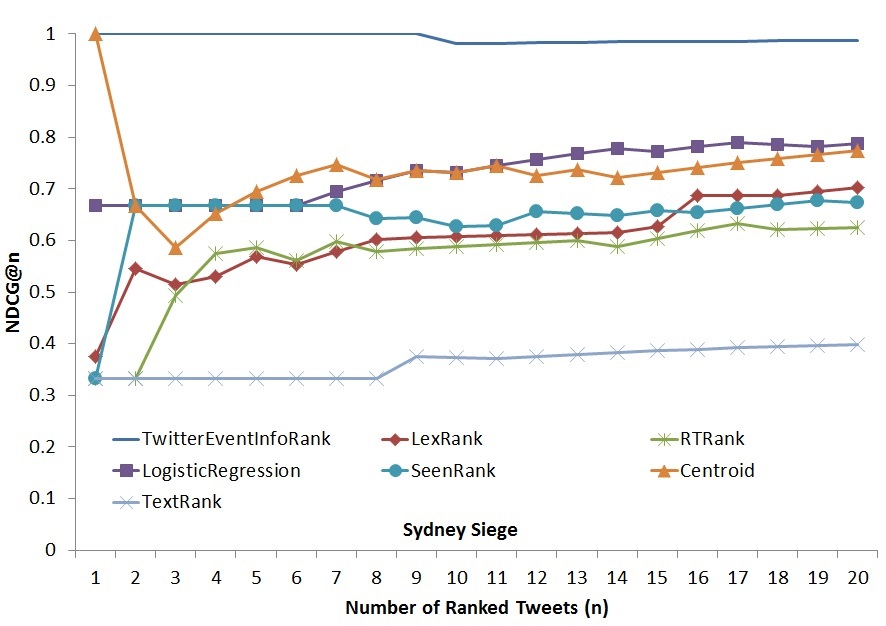
\includegraphics[height=4.5in,width=6in]{Figures/Chapter4Figures/SydneySiegeEventIdentityInfoRankPerformance.jpg}
\caption{\small Performance comparison of ranking techniques using NDCG scores.}
\label{sydneysiegendcg}
\end{figure}


\begin{table}[htbp]
\centering
\caption{Avg IIC scores and total avg scores of annotations for Millions March NYC event.}
\label{avgiicMillionsMarchNyc}
\begin{tabular}{|c|c|c|}
\hline
\textbf{\begin{tabular}[c]{@{}c@{}}Millions March \\ NYC\end{tabular}} & \textbf{IIC} & \textbf{\begin{tabular}[c]{@{}c@{}}Total Avg \\ Score (1-3)\end{tabular}} \\ \hline
\textbf{\begin{tabular}[c]{@{}c@{}}Top 50 event-specific\\ informative Hashtags\end{tabular}} & 0.786 & 1.980 \\ \hline
\textbf{\begin{tabular}[c]{@{}c@{}}Top 50 event-specific\\ informative Text Units\end{tabular}} & 0.880 & 1.320 \\ \hline
\textbf{\begin{tabular}[c]{@{}c@{}}Top 50 event-specific\\ informative URLs\end{tabular}} & 0.926 & 2.560 \\ \hline
\textbf{\begin{tabular}[c]{@{}c@{}}Top 50 event-specific\\ informative Users\end{tabular}} & 0.700 & 2.386 \\ \hline
\textbf{\begin{tabular}[c]{@{}c@{}}Top 100 event-specific\\ informative Tweets\end{tabular}} & 0.760 & 2.59 \\ \hline
\end{tabular}
\end{table}



\begin{table}[htbp]
\centering
\caption{Avg IIC scores and total avg scores of annotations for Sydney Siege event.}
\label{avgiicSydneySiege}
\begin{tabular}{|c|c|c|}
\hline
\textbf{Sydney Siege} & \textbf{IIC} & \textbf{\begin{tabular}[c]{@{}c@{}}Total Avg\\ Score (1-3)\end{tabular}} \\ \hline
\textbf{\begin{tabular}[c]{@{}c@{}}Top 50 event-specific\\ informative Hashtags\end{tabular}} & 0.880 & 2.027 \\ \hline
\textbf{\begin{tabular}[c]{@{}c@{}}Top 50 event-specific\\ informative Text Units\end{tabular}} & 0.986 & 1.487 \\ \hline
\textbf{\begin{tabular}[c]{@{}c@{}}Top 50 event-specific\\ informative URLs\end{tabular}} & 0.893 & 2.413 \\ \hline
\textbf{\begin{tabular}[c]{@{}c@{}}Top 50 event-specific\\ informative Users\end{tabular}} & 0.646 & 2.353 \\ \hline
\textbf{\begin{tabular}[c]{@{}c@{}}Top 100 event-specific\\ informative Tweets\end{tabular}} & 0.83 & 2.62 \\ \hline
\end{tabular}
\end{table}

\begin{figure}[htbp]
\centering
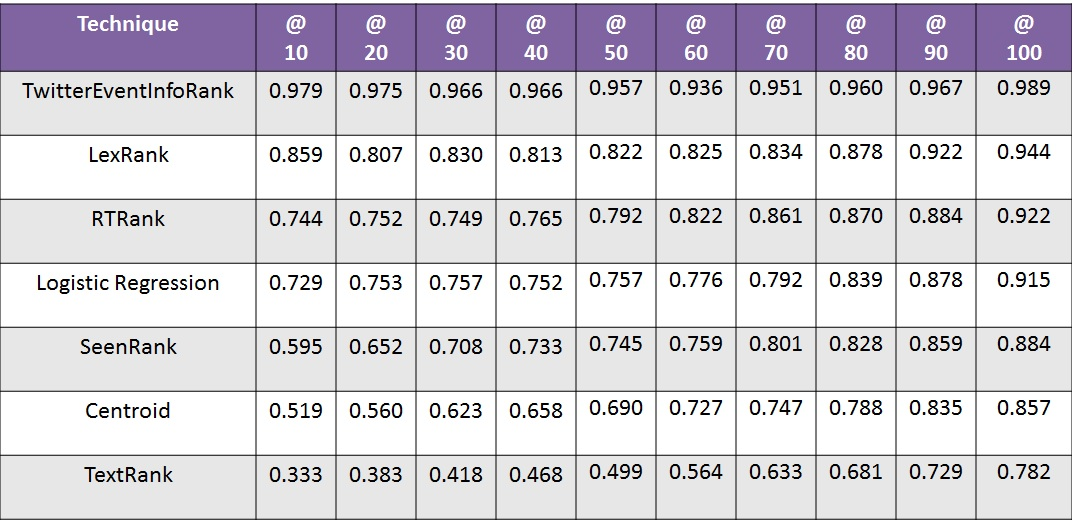
\includegraphics[height=3.5in,width=5.5in]{Figures/millionsmarchnycndcg.jpg}
\caption{\small Performance comparison of ranking techniques using NDCG scores.}
\label{millionsmarchndcg}
\end{figure}

\begin{figure}[htbp]
\centering
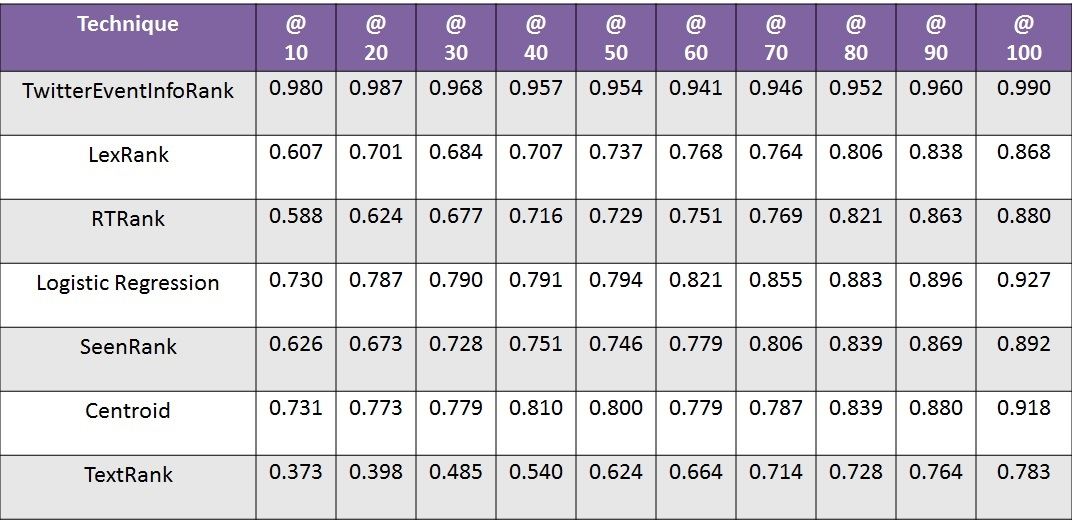
\includegraphics[height=3.5in,width=5.5in]{Figures/sydneysiegendcg.jpg}
\caption{\small Performance comparison of ranking techniques using NDCG scores.}
\label{sydneysiegendcg}
\end{figure}

\begin{figure}[htbp]
\centering
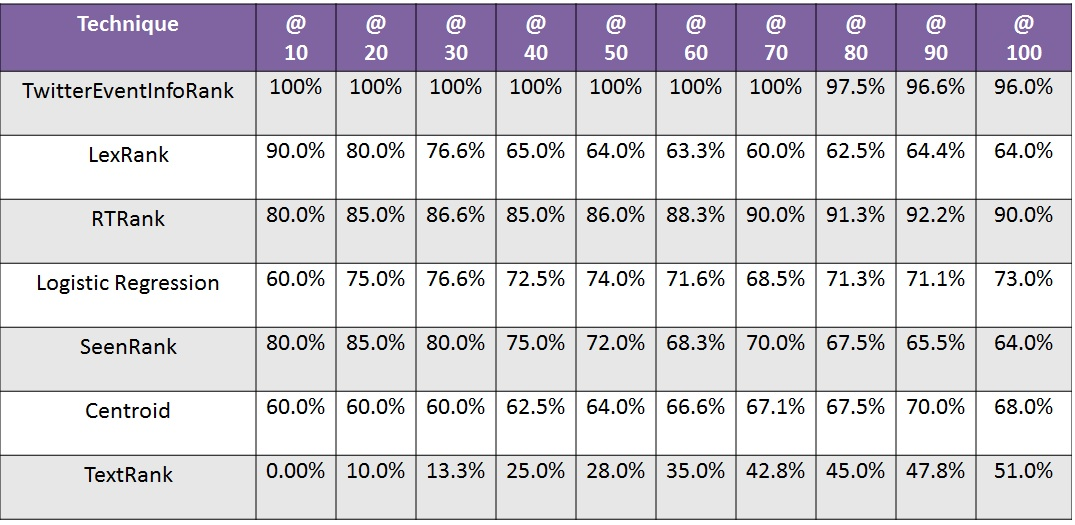
\includegraphics[height=3.5in,width=5.5in]{Figures/millionsmarchnycprecision.jpg}
\caption{\small Performance comparison of ranking techniques using precision scores.}
\label{millionsmarchnycprecision}
\end{figure}

\begin{figure}[htbp]
\centering
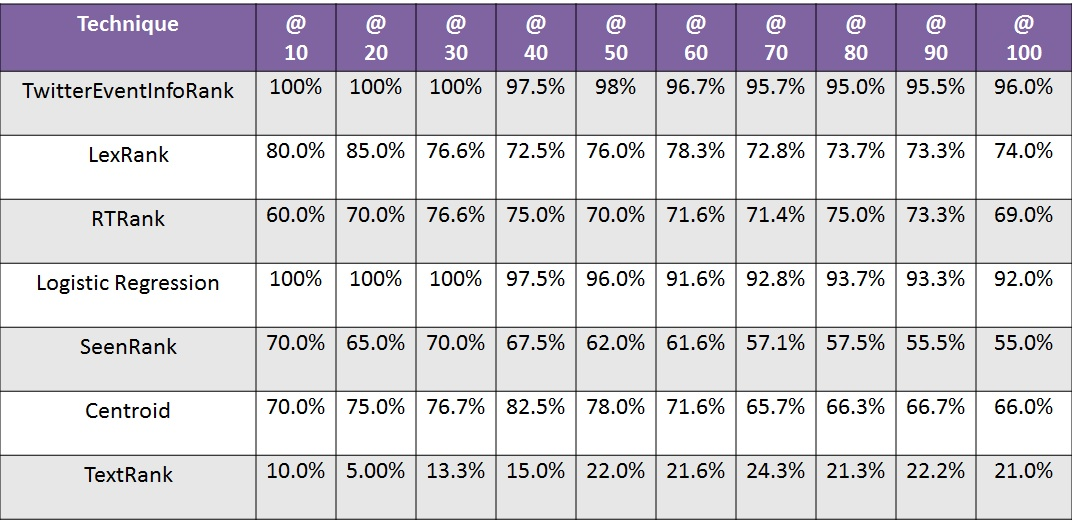
\includegraphics[height=3.5in,width=5.5in]{Figures/sydneysiegeprecision.jpg}
\caption{\small Performance comparison of ranking techniques using precision scores.}
\label{sydneysiegeprecision}
\end{figure}
